\documentclass[aspectratio=169,10pt]{beamer}
% Course-local adaptation of the copied Sorbonne Beamer reference assets.
% The files in template/assets/ are preserved verbatim from the reference copy.
\usepackage[T1]{fontenc}
\usepackage[utf8]{inputenc}
\usepackage{lmodern}
\usepackage{amsmath,amssymb,mathtools}
\usepackage{booktabs}
\usepackage{graphicx}
\usepackage{tikz}
\usetikzlibrary{arrows.meta,positioning,calc}
\usepackage{ragged2e}
\usepackage{hyperref}
\definecolor{bleu}{RGB}{0,129,188}
\definecolor{rouge}{RGB}{238,50,78}
\definecolor{orange}{RGB}{255,100,0}
\definecolor{vert}{RGB}{0,157,87}
\definecolor{dp}{RGB}{181,73,60}
\usetheme{Frankfurt}
\useoutertheme[subsection=false,shadow]{miniframes}
\usepackage{template/assets/beamercolorthemeEwen}
\usepackage{template/assets/beamerouterthemeEwen}
\usepackage{template/assets/beamerhighlight}
\usefonttheme{serif}
\setbeamerfont{title like}{shape=\scshape}
\setbeamerfont{frametitle}{shape=\scshape}
\setbeamercolor{frametitle}{fg=dp,bg=white}
\setbeamercolor{structure}{fg=black}
\setbeamercolor{alerted text}{fg=dp}
\setbeamertemplate{navigation symbols}{}
\setbeamertemplate{items}[triangle]
\setbeamertemplate{footline}{%
  \leavevmode\hbox{\begin{beamercolorbox}[wd=1\paperwidth,ht=2.25ex,dp=1ex,center]{title in head/foot}
  \hfill\hspace*{8em}\insertshorttitle\hspace*{2em}\insertframenumber{} / \inserttotalframenumber\hspace*{1ex}
  \end{beamercolorbox}}\vskip0pt}
\newcommand{\key}[1]{\textcolor{dp}{\textbf{#1}}}
\AtBeginSection[]{\begin{frame}{Plan}\tableofcontents[currentsection,hideallsubsections]\end{frame}}

\title[BTM -- Session 3]{Maximum Likelihood Estimation}
\subtitle{State-space models, filtering and DSGE likelihoods}
\author[Gauthier Vermandel]{Gauthier Vermandel}
\institute{Paris-Dauphine -- PSL}
\date{19 November 2026}
\begin{document}
\begin{frame}\titlepage\end{frame}
\begin{frame}{Session objective}\begin{itemize}\item Express a solved DSGE model as a state-space system.\item Evaluate the likelihood with the Kalman filter.\item Interpret estimates alongside identification and diagnostics.\end{itemize}\vfill\key{Handout:} Chapter 3 \quad \key{Code:} \texttt{chap3/codes/}\end{frame}
\section{State-space representation}
\begin{frame}{From model solution to observations}
\[\underbrace{s_t}_{\text{state}}=T s_{t-1}+R\varepsilon_t,\qquad\underbrace{y_t}_{\text{data}}=Zs_t+d+\eta_t.\]
\begin{itemize}\item The transition equation propagates latent states.\item The measurement equation links the model to transformed data.\item Measurement error \(\eta_t\) is an economic and statistical assumption.\end{itemize}\end{frame}
\begin{frame}{Data transformations are part of the measurement equation}\centering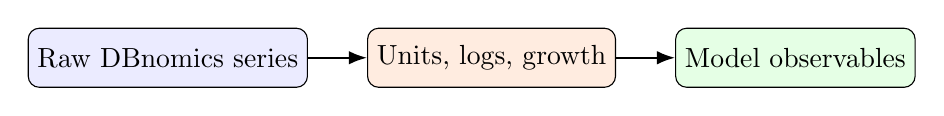
\begin{tikzpicture}[node distance=.75cm,>=Latex,every node/.style={draw,rounded corners,align=center,minimum width=2.2cm,minimum height=.75cm}]
\node[fill=blue!8] (raw) {Raw DBnomics series};\node[fill=orange!12,right=of raw] (tr) {Units, logs, growth};\node[fill=green!10,right=of tr] (obs) {Model observables};\draw[->,thick] (raw)--(tr);\draw[->,thick] (tr)--(obs);\end{tikzpicture}
\vfill\key{Always record:} provider, dataset, series, frequency, sample, missing values and transformation.\end{frame}
\section{Likelihood}
\begin{frame}{The likelihood decomposes prediction errors}
At each date, the Kalman filter delivers a forecast error \(v_t\) and covariance \(F_t\):
\[\log L(\theta)=-\frac12\sum_t\left[\log|F_t|+v_t'F_t^{-1}v_t+n_y\log(2\pi)\right].\]
\begin{itemize}\item Parameters affect both the forecast and its uncertainty.\item Missing observations can be handled systematically.\item The filter turns a dynamic model into an evaluable criterion.\end{itemize}\end{frame}
\begin{frame}{Kalman filter: intuition}\centering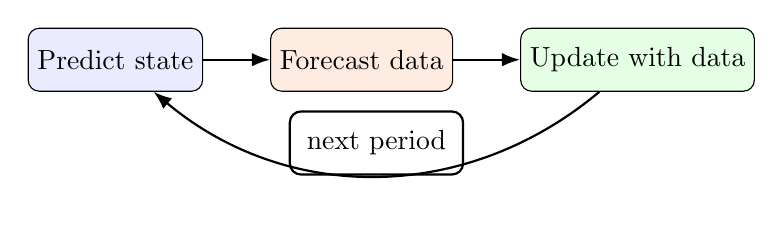
\begin{tikzpicture}[node distance=.85cm,>=Latex,every node/.style={draw,rounded corners,align=center,minimum width=2.2cm,minimum height=.8cm}]
\node[fill=blue!8] (p) {Predict state};\node[fill=orange!12,right=of p] (f) {Forecast data};\node[fill=green!10,right=of f] (u) {Update with data};\draw[->,thick] (p)--(f);\draw[->,thick] (f)--(u);\draw[->,thick,bend left=40] (u) to node[above]{next period} (p);\end{tikzpicture}
\vfill The gain balances model-implied uncertainty against measurement uncertainty.\end{frame}
\section{Estimation}
\begin{frame}{Maximum likelihood workflow}\begin{enumerate}\item Specify model, observables and parameter domain.\item Build the state-space solution and evaluate \(\log L(\theta)\).\item Optimize from multiple informed starting values.\item Inspect convergence, curvature, residuals and economic plausibility.\end{enumerate}\end{frame}
\begin{frame}{A numerical optimum is not the end}\begin{columns}[T]\begin{column}{.49\textwidth}\begin{block}{Check}\begin{itemize}\item optimization status\item parameter bounds\item Hessian / standard errors\item forecast errors\end{itemize}\end{block}\end{column}\begin{column}{.49\textwidth}\begin{block}{Question}\centering Is the likelihood informative about this parameter, or is the result driven by a restriction?\end{block}\end{column}\end{columns}\end{frame}
\section{Takeaways}
\begin{frame}{Takeaways and preparation}\begin{itemize}\item Estimation begins with the measurement equation, not the optimizer.\item The Kalman filter evaluates likelihoods recursively.\item Diagnostics distinguish a computational answer from credible inference.\end{itemize}\vfill\key{Before Session 4:} inspect the observables and prior choices in \texttt{RBC\_estim.mod}.\end{frame}
\end{document}
